\documentclass[conference]{IEEEtran}
\IEEEoverridecommandlockouts
\usepackage{cite}
\usepackage{amsmath,amssymb}
\usepackage{graphicx}
\usepackage{booktabs}
\usepackage{xcolor}
\usepackage{url}
\usepackage[hidelinks]{hyperref}
\graphicspath{{figures/}}
\newcommand{\todo}[1]{\textcolor{red}{[#1]}}

\begin{document}

\title{What Does the Market Pay For? A Tuned Neural-Network Fair-Value Model for Indian Large Caps}

\author{
\IEEEauthorblockN{Sanket Gore, Milind Gauns, Shakthi Keshavan}
\IEEEauthorblockA{Goa Institute of Management\\
Big Data Analytics\\
Student IDs: \{B2026147, B2026134, B2026149\}\\
Email: \{sanket.gore2026b, milind.gauns2026b, shakthi.k2026b\}@gim.ac.in}
}

\maketitle

\begin{abstract}
Indian large caps trade at very different multiples of book value: between 2017 and 2025 the median consumer-discretionary company in our sample traded at about 13 times book, the median metals or oil and gas company at 1.5 times. We ask how much of this spread a company's own accounts explain, and whether the part they leave unexplained predicts returns. Using CMIE Prowess data for 141 non-financial NIFTY~200 companies (1,102 company-years), we predict each company's log price-to-book ratio on 30~June from ten accounting ratios, its sector and three price-based inputs. A Ridge regression, a Random Forest, XGBoost and a multilayer perceptron (MLP) are tuned and tested walk-forward over 2019--2025, so every prediction uses only earlier years. The tuned MLP explains 70.1\% of the out-of-sample variation, against 68.3\% for XGBoost, 64.1\% for Random Forest and 56.4\% for Ridge; averaging the network over ten random seeds raises this to 70.5\%. The tuning study shows that the L2 penalty and network width matter most, while the activation function and optimiser matter little. Three results qualify the network's lead. Last year's own P/B predicts better than any model (81.2\%); for companies the model has never seen, XGBoost generalises best (61.0\% against 57.7\% for the MLP); and the model's ``cheap'' stocks did not outperform its ``expensive'' ones over the next 12 months (mean rank correlation $-0.06$). The unexplained part of valuation is a persistent company premium rather than a short-lived pricing error. The pipeline is deterministic, and rerunning it on the frozen data reproduces every reported number.
\end{abstract}

\begin{IEEEkeywords}
Relative valuation, price-to-book, neural networks, hyperparameter tuning, walk-forward validation, reproducibility, Indian equity market
\end{IEEEkeywords}

\section{Introduction}
Valuation by multiples is the most widely used method in equity practice because it is quick to apply. Its weak point is the choice of the multiple itself. Analysts usually select a handful of comparable companies and apply judgement, although the reasons one company trades at a premium to another (higher returns on capital, faster growth, lower risk, stronger brands) are rarely quantified. The spread is large in India: over our sample period, price-to-book (P/B) ratios ranged from about 0.3 to more than 100.

This study replaces the judgement with a model estimated across companies and years. A model that learns which fundamentals the market rewards has three practical uses: it provides a fair multiple for any listed company, it flags stocks that trade far above or below what their fundamentals justify, and it gives a starting multiple for valuing an unlisted business against listed peers.

The study also has two methodological aims. The first is reproducibility: every step, from reading the raw data to training the models, is deterministic, so rerunning the code on the same data returns the same numbers. The second is to examine the neural network itself rather than treat it as a black box, by measuring its sensitivity to hyperparameters, its dependence on the random seed, the inputs it relies on, and how well it generalises to companies it has not seen.

\subsection{Scope and Objectives}
\begin{itemize}
\item To measure how much of the cross-section of P/B ratios among Indian large caps is explained by accounting fundamentals, and whether a tuned neural network explains more than a linear model or tree ensembles.
\item To study the network's tuning: which hyperparameters matter, how stable the result is across seeds, and which inputs carry the signal.
\item To test whether the model can value companies absent from its training data.
\item To test whether the gap between actual and fair valuation predicts returns over the following 12 months.
\end{itemize}

\section{Related Work}
The link between accounting numbers and market value is well established. Ohlson~\cite{ohlson1995} wrote firm value as a function of book value and expected abnormal earnings, which implies that P/B rises with the expected return on equity relative to the cost of capital. Penman~\cite{penman1996} showed how P/B and P/E jointly reflect current profitability and expected growth. These results set the expectation for this study: return on equity and growth should raise P/B, and risk should lower it.

Practitioners apply this logic through multiples. Bhojraj and Lee~\cite{bhojraj2002} replaced industry peer groups with a ``warranted multiple'' predicted by regression on profitability, growth and risk, and found that it selected better comparable firms. Damodaran~\cite{damodaran2012} presents the same reasoning in textbook form. Rhodes-Kropf, Robinson and Viswanathan~\cite{rhodes2005} decomposed market-to-book into a component explained by fundamentals and a residual interpreted as misvaluation, which corresponds to the mispricing measure used here.

Machine learning has been applied to both valuation and return prediction. Gu, Kelly and Xiu~\cite{gu2020} found that neural networks and tree ensembles improve on linear models for predicting US stock returns. Geertsema and Lu~\cite{geertsema2023} used gradient boosting for relative valuation on US data and found that machine-learned multiples were more accurate than traditional ones and that the gap between price and predicted value forecast the next month's return. Grinsztajn et al.~\cite{grinsztajn2022} reported that tree-based models usually outperform deep learning on tabular data, which is why we benchmark the network against XGBoost~\cite{chen2016} and Random Forest~\cite{breiman2001}.

On method, Bergstra and Bengio~\cite{bergstra2012} showed that random search finds good hyperparameters more efficiently than grid search; Bouthillier et al.~\cite{bouthillier2021} showed that the random seed alone can change measured performance by more than the gap between methods; and Lakshminarayanan et al.~\cite{lakshminarayanan2017} showed that averaging networks trained from different initialisations improves accuracy and stability. All three shaped our tuning study.

\section{Methodology}
\subsection{Data}
\textbf{Source and universe.} All data were taken from CMIE Prowess in November 2026. The universe is the current NIFTY~200 index, restricted to non-financial companies (148 firms). Two companies that Prowess classifies as non-financial but whose business is financial (a stock broker and a payments company) were removed.

\textbf{Accounts.} For each company we downloaded Prowess \emph{Abridged Annual Financials}, FY2011--FY2026, on both a consolidated and a standalone basis. For each company-year we use consolidated figures where available (1,030 of the final 1,102 observations) and standalone figures otherwise. Ratios that require history, namely ROE on average equity, three-year sales growth and ROE stability, are computed within one basis, so a change of basis cannot create an artificial jump. Consolidated statements became compulsory only from FY2015 under the Companies Act, 2013; where the consolidated history is too short, the standalone growth rate and ROE stability are used. Accounting periods other than 12 months, caused by changes in year end, are scaled to 12 months.

\textbf{Prices.} Monthly NSE adjusted closing prices (corrected for splits, bonuses and rights issues), monthly average market capitalisation and the NIFTY~50 index were downloaded for January 2010 to October 2026.

\textbf{Timing.} Indian companies publish annual results within about two months of the year end. Each year's accounts are therefore matched to the first 30~June at least 60 days after the year end (the \emph{formation date}), so the model uses only information that investors already had.

\textbf{Target and inputs.} The target is the natural log of P/B, defined as June's average market capitalisation divided by the latest net worth. The inputs are listed in Table~\ref{tab:features}. Each ratio is capped at fixed limits chosen in advance, for example ROE between $-100\%$ and $150\%$ and debt-to-equity at 10, so that a few extreme values cannot dominate the fit.

\textbf{Sample rules.} Prowess's abridged statements are sparse before FY2014, so three-year ratios are available from the 2017 formation date onwards; the sample therefore covers 2017--2025. To ensure that every observation represents a large company at the time, and not only today, a company enters a year only if its market capitalisation on the formation date is at least Rs.~5,000 crore. Observations with P/B outside 0.05--200, all caused by near-zero or negative book value, are excluded. The final sample contains 1,102 company-years from 141 companies, between 111 and 139 per year. The 66 NSE industry labels are grouped into 12 sectors. Fig.~\ref{fig:sector} shows the spread of valuations by sector.

\begin{table}[t]
\caption{Model inputs (all from data available on the formation date)}
\label{tab:features}
\centering
\footnotesize
\begin{tabular}{@{}lp{5.3cm}@{}}
\toprule
Input & Definition \\
\midrule
\multicolumn{2}{@{}l}{\emph{Fundamentals (latest annual accounts)}}\\
ROE & Net profit / average net worth \\
Operating margin & (PBT + interest + depreciation $-$ other income) / sales \\
Sales growth & 3-year compound growth in sales \\
Debt/equity & Total borrowings / net worth \\
Interest cover & $\log(1 + (\text{PBT} + \text{interest})/\text{interest})$, capped at 100 \\
Asset turnover & Sales / total assets \\
Payout & Dividends / net profit, capped at 1.5 \\
Cash conversion & Operating cash flow / net profit \\
ROE stability & Standard deviation of ROE over 3 years \\
Size & $\log$(sales) \\
Sector & 12 sector indicators \\
\midrule
\multicolumn{2}{@{}l}{\emph{Market (up to the formation date)}}\\
Momentum & $\log(1 + \text{12-month price return})$ \\
Volatility & Annualised s.d.\ of monthly returns, 24 months \\
Beta & Beta to the NIFTY~50, 36 months \\
\bottomrule
\end{tabular}
\end{table}

\begin{figure}[t]
\centering
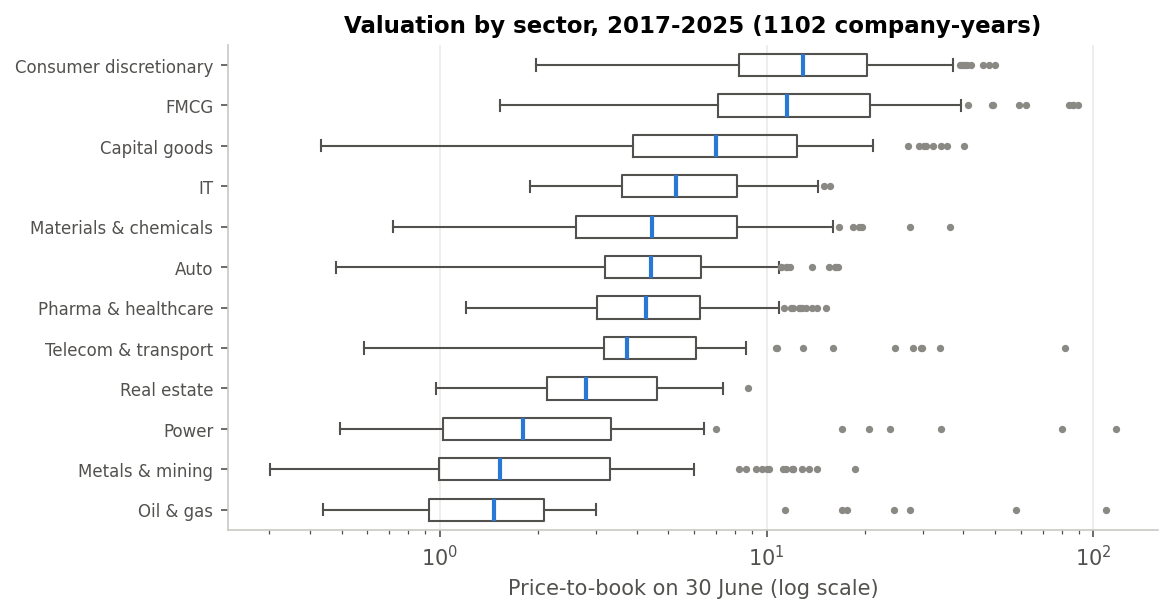
\includegraphics[width=\columnwidth]{fig1_pb_by_sector.png}
\caption{Distribution of P/B on 30~June by sector, 2017--2025 (log scale; 1,102 company-years).}
\label{fig:sector}
\end{figure}

\subsection{Models and Tuning}
All models share one pipeline of median imputation, standardisation and the estimator. We compare five approaches:
\begin{itemize}
\item \textbf{Ridge regression}~\cite{hoerl1970}, the linear valuation regression of~\cite{bhojraj2002} with an L2 penalty chosen from seven values;
\item \textbf{Random Forest}~\cite{breiman2001} with 300 trees, tuned over features per split and leaf size;
\item \textbf{XGBoost}~\cite{chen2016}, tuned over tree depth, learning rate and number of trees;
\item \textbf{MLP}, scikit-learn's multilayer perceptron~\cite{pedregosa2011}, tuned by seeded random search~\cite{bergstra2012} over architecture (one or two hidden layers of 4 to 32 neurons), activation (ReLU or tanh), L2 penalty ($10^{-3}$ to 30), optimiser (Adam or L-BFGS) and learning rate;
\item \textbf{Naive benchmark}: the company's own log P/B in the previous year.
\end{itemize}

\textbf{Walk-forward testing.} For each test year from 2019 to 2025, every model is tuned and trained only on earlier years and then predicts that year's P/B, giving 879 out-of-sample predictions. Within each training set, candidate settings are scored on the last three training years, one at a time, each time training only on the years before it. This expanding-window validation respects time order. The MLP search evaluates 30 settings in each step.

\textbf{Determinism.} Every random draw uses a fixed seed (42), and all models run on a single thread, so floating-point operations occur in the same order on every run. The raw files are checked against SHA-256 checksums before any computation.

\subsection{Evaluation}
Valuation accuracy is measured by three statistics: out-of-sample R\textsuperscript{2} against a prediction equal to the training-period mean; RMSE of log P/B; and the mean within-year Spearman rank correlation between predicted and actual P/B. We also test generalisation to new companies with five-fold cross-validation grouped by company, so that each company is predicted by a model trained only on the others.

\textbf{Investment test.} On each formation date from 2019 to 2025, \emph{mispricing} is defined as actual minus predicted log P/B, using the out-of-sample prediction. Stocks are sorted into quintiles by cheapness. We report the Spearman rank correlation between cheapness and the next 12-month price return (the information coefficient, IC) and the average return of each quintile.

\section{Results}
\subsection{How Well Fundamentals Explain Valuations}
Table~\ref{tab:wf} reports the walk-forward results. The tuned MLP is the most accurate model, explaining 70.1\% of the out-of-sample variation in log P/B with an RMSE of 0.577. XGBoost follows closely at 68.3\%, Random Forest reaches 64.1\% and Ridge 56.4\%. The rank correlations show the same ordering, apart from a near tie between the MLP and XGBoost. An RMSE of 0.577 means that a typical prediction lies within a factor of about 1.8 of the actual P/B, on a sample where P/B ranges over more than two orders of magnitude. By year (Table~\ref{tab:year}), the MLP has a lower RMSE than Ridge in six of seven years and lower than XGBoost in five.

\begin{table}[t]
\caption{Walk-forward results, 2019--2025 (879 predictions)}
\label{tab:wf}
\centering
\footnotesize
\begin{tabular}{@{}lccc@{}}
\toprule
Model & OOS R\textsuperscript{2} & RMSE (log P/B) & Rank corr. \\
\midrule
Ridge & 0.564 & 0.696 & 0.787 \\
Random Forest & 0.641 & 0.632 & 0.826 \\
XGBoost & 0.683 & 0.594 & \textbf{0.843} \\
MLP (tuned) & \textbf{0.701} & \textbf{0.577} & 0.842 \\
\midrule
Naive (last year's P/B)$^{a}$ & 0.812 & 0.455 & 0.931 \\
\bottomrule
\multicolumn{4}{@{}l}{\scriptsize $^{a}$860 predictions; requires a P/B in the previous year.}
\end{tabular}
\end{table}

\begin{table}[t]
\caption{RMSE of log P/B by test year}
\label{tab:year}
\centering
\footnotesize
\begin{tabular}{@{}lcccc@{}}
\toprule
Year & Ridge & Random Forest & XGBoost & MLP \\
\midrule
2019 & 0.489 & 0.495 & \textbf{0.440} & 0.511 \\
2020 & 0.610 & 0.586 & 0.517 & \textbf{0.486} \\
2021 & 0.629 & 0.706 & 0.640 & \textbf{0.590} \\
2022 & 0.785 & 0.748 & 0.670 & \textbf{0.640} \\
2023 & 0.738 & 0.541 & 0.531 & \textbf{0.465} \\
2024 & 0.775 & 0.671 & 0.623 & \textbf{0.584} \\
2025 & 0.752 & \textbf{0.623} & 0.668 & 0.699 \\
\bottomrule
\end{tabular}
\end{table}

The naive benchmark outperforms every model, explaining 81.2\% of the variation. This reflects the market more than the models: large-cap valuations are persistent, and whatever supports a company's multiple in one year largely carries into the next. The fundamentals model addresses a different question, namely what multiple a given set of accounts justifies, which is the relevant question for a company without a price history. Fig.~\ref{fig:fair} plots predicted against actual P/B; the points follow the diagonal across two orders of magnitude.

\begin{figure}[t]
\centering
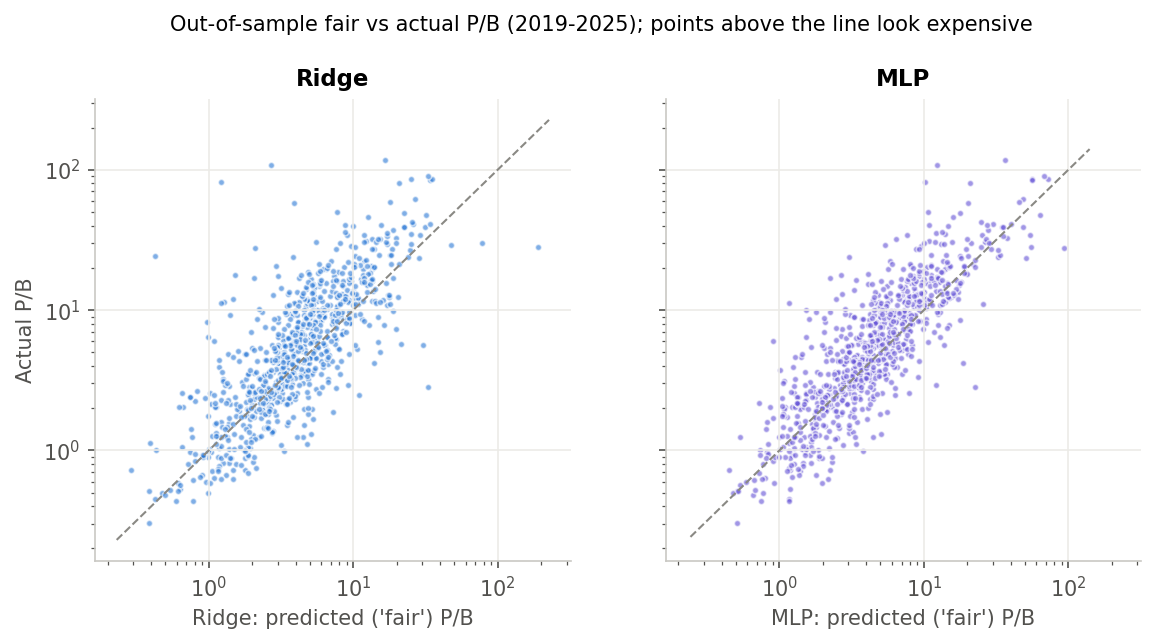
\includegraphics[width=\columnwidth]{fig3_fair_vs_actual.png}
\caption{Out-of-sample predicted (``fair'') versus actual P/B, 2019--2025, log scales. Points above the line traded above the model's fair value.}
\label{fig:fair}
\end{figure}

\subsection{Tuning Study: Which Settings Matter}
To measure the network's sensitivity, we evaluated 60 random settings once on the full sample, validating on its last three years (Fig.~\ref{fig:tuning}). This search is descriptive; the walk-forward results above never used it.

\begin{figure*}[t]
\centering
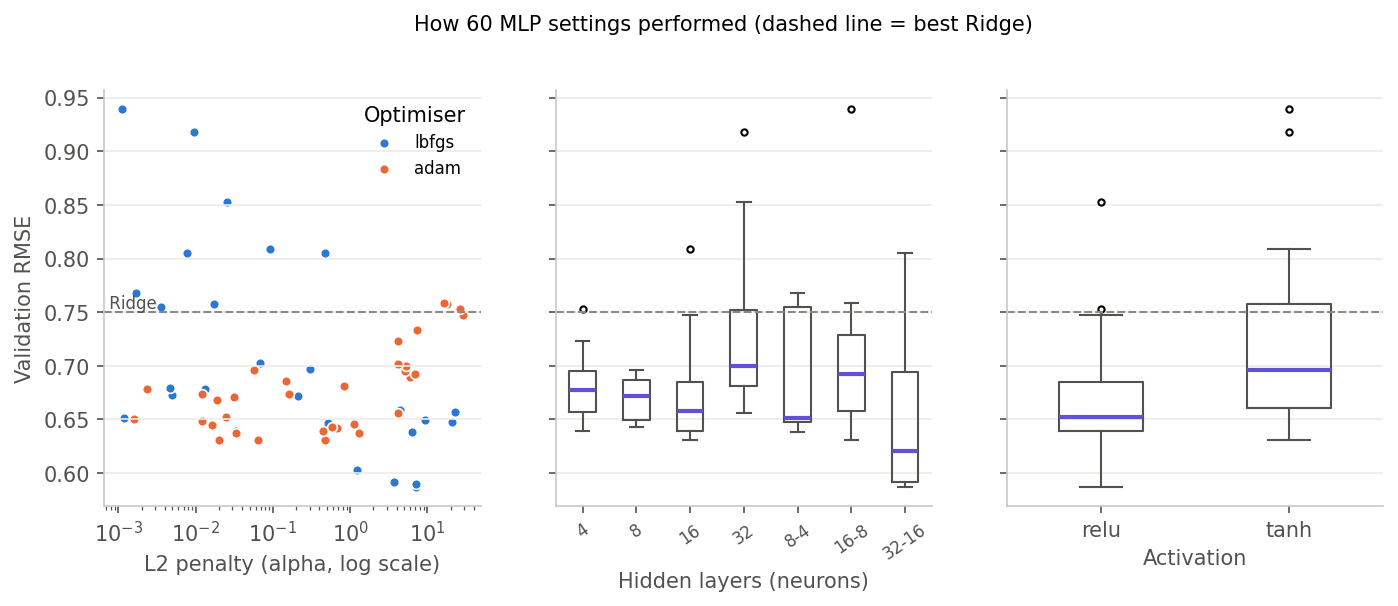
\includegraphics[width=0.85\textwidth]{fig4_tuning_study.png}
\caption{Validation RMSE of 60 MLP settings by L2 penalty and optimiser (left), architecture (centre) and activation (right). The dashed line marks the best Ridge model.}
\label{fig:tuning}
\end{figure*}

The best setting reached a validation RMSE of 0.587, against 0.750 for the best Ridge model; 48 of the 60 settings outperformed Ridge, and the median setting scored 0.673. The four best settings share the same structure: a 32--16 network with ReLU activation, the L-BFGS optimiser and an L2 penalty between 1.2 and 7.1.

\textbf{Regularisation.} Settings with an L2 penalty between 1 and 10 had the lowest median RMSE (0.656). With almost no penalty (below 0.01) the median rose to 0.717, and with a heavy penalty (above 10) to 0.750, no better than Ridge. Too little regularisation lets the network over-fit about 1,000 observations; too much reduces it to a nearly linear function.

\textbf{Architecture and activation.} The 32--16 network had the lowest median RMSE (0.620), and the other architectures ranged from 0.651 to 0.700. ReLU outperformed tanh (median 0.652 against 0.697). The choice of optimiser made almost no difference (0.673 for both).

\subsection{Seed Sensitivity}
Because a neural network starts from random weights, we retrained each model with ten seeds while keeping the hyperparameters selected in the walk-forward run (Fig.~\ref{fig:seeds}, Table~\ref{tab:robust}). The MLP's R\textsuperscript{2} ranged from 0.677 to 0.697 (mean 0.687, standard deviation 0.007). The headline value of 0.701 from seed 42 lies just above this range, so the mean of 0.687 is the more representative estimate. XGBoost ranged from 0.671 to 0.684 and Random Forest from 0.638 to 0.644. The ranges of the MLP and XGBoost overlap, so the network's lead over XGBoost from a single training run is small. Averaging the ten MLPs' predictions, however, gives 0.705, above every individual run of any model, which makes the seed ensemble the most accurate model in the study.

\begin{figure}[t]
\centering
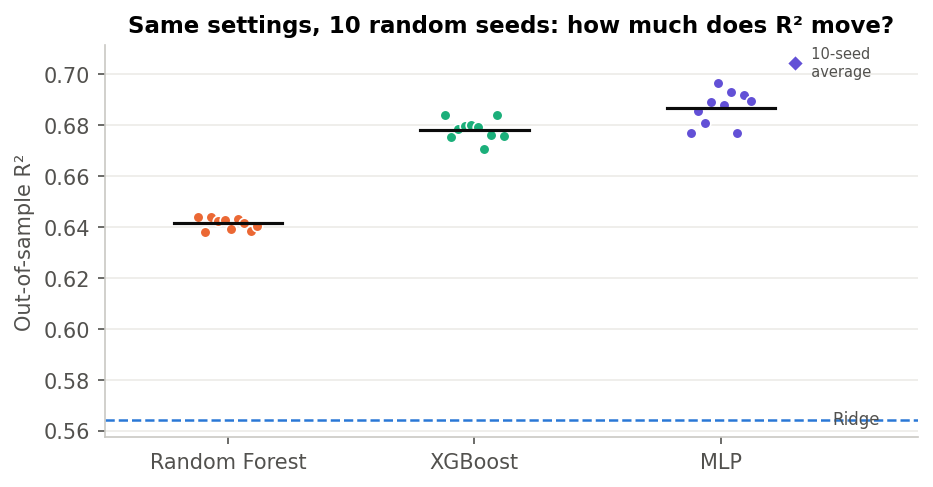
\includegraphics[width=\columnwidth]{fig5_seed_sensitivity.png}
\caption{Out-of-sample R\textsuperscript{2} for ten random seeds with fixed hyperparameters. Black lines mark the mean; the diamond is the average of the ten MLPs. The dashed line is Ridge.}
\label{fig:seeds}
\end{figure}

\begin{table}[t]
\caption{Seed sensitivity, input ablation and generalisation (R\textsuperscript{2})}
\label{tab:robust}
\centering
\footnotesize
\begin{tabular}{@{}lcccc@{}}
\toprule
\multicolumn{5}{@{}l}{\emph{(a) Ten seeds, fixed hyperparameters}} \\
 & Mean & Std. & Min & Max \\
\midrule
Random Forest & 0.641 & 0.002 & 0.638 & 0.644 \\
XGBoost & 0.678 & 0.004 & 0.671 & 0.684 \\
MLP & 0.687 & 0.007 & 0.677 & 0.697 \\
MLP, 10-seed average & 0.705 & -- & -- & -- \\
Ridge (no randomness) & 0.564 & 0 & -- & -- \\
\midrule
\multicolumn{5}{@{}l}{\emph{(b) Input ablation (walk-forward)}} \\
 & Ridge & XGBoost & MLP & \\
\midrule
Fundamentals only & 0.530 & 0.643 & 0.630 & \\
Market only & 0.064 & 0.085 & 0.053 & \\
Both & 0.564 & 0.683 & 0.701 & \\
\midrule
\multicolumn{5}{@{}l}{\emph{(c) Companies not in the training data}} \\
 & Ridge & XGBoost & MLP & \\
\midrule
R\textsuperscript{2} & 0.560 & \textbf{0.610} & 0.577 & \\
RMSE & 0.676 & \textbf{0.637} & 0.663 & \\
\bottomrule
\end{tabular}
\end{table}

\subsection{Which Inputs Carry the Signal}
The ablation in Table~\ref{tab:robust}(b) shows that fundamentals explain 53--64\% of the variation on their own, while the three price-based inputs alone explain at most 9\%. Combining them adds between 3 and 7 points, with the largest gain for the MLP, which appears to make better use of interactions between the two groups. With fundamentals alone, XGBoost is slightly ahead of the MLP (0.643 against 0.630).

Permutation importance~\cite{fisher2019} for the MLP (Fig.~\ref{fig:imp}) ranks asset turnover first, followed by size (larger companies trade at lower multiples), ROE, debt-to-equity and the sector indicators for oil and gas (a discount) and consumer discretionary (a premium). Asset turnover partly reflects business model: IT and consumer companies run on few physical assets, so they generate more sales per rupee of assets and carry a smaller book value, both of which raise P/B.

\begin{figure}[t]
\centering
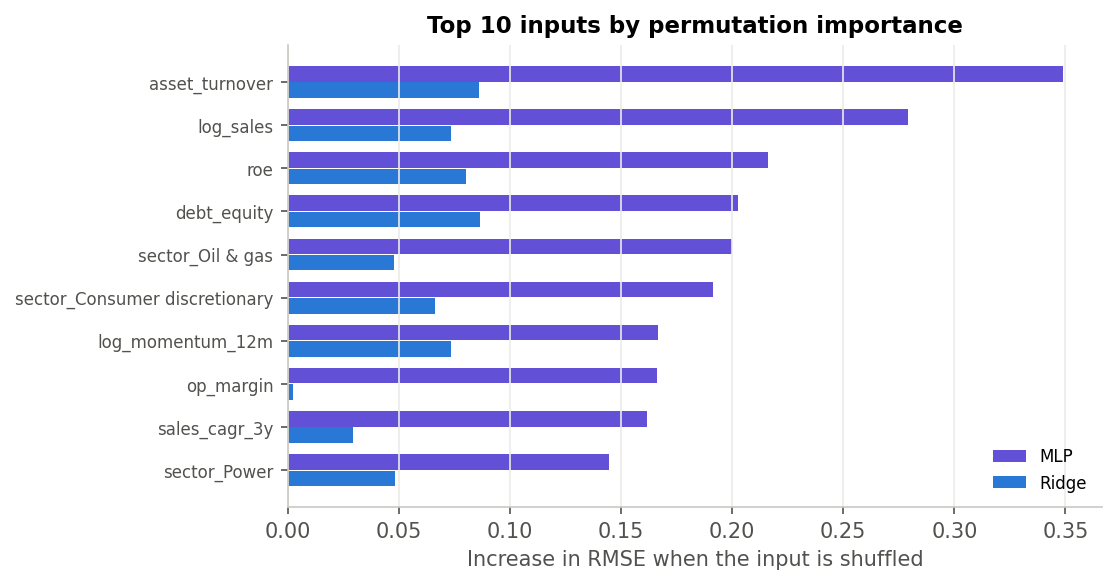
\includegraphics[width=\columnwidth]{fig6_importance.png}
\caption{Permutation importance: increase in RMSE when each input is shuffled (top ten inputs, full-sample models).}
\label{fig:imp}
\end{figure}

The partial dependence plots~\cite{friedman2001} in Fig.~\ref{fig:pdp} show how fair P/B responds to individual inputs. Both models raise fair P/B from about 4.0 to 6.7 as ROE rises from zero to 45\%, consistent with valuation theory~\cite{ohlson1995,penman1996}, and both reward sales growth. Operating margin is where the two models differ most. The MLP raises fair P/B from about 4.0 to 6.6 across the observed range, while Ridge moves only from 4.7 to 5.3, because in a linear model margin and ROE largely substitute for each other. Both models assign a positive slope to debt-to-equity. This is plausible in a P/B setting, since for a given return on assets, leverage raises ROE and reduces book equity, but it means the model captures the leverage effect rather than financial risk.

\begin{figure*}[t]
\centering
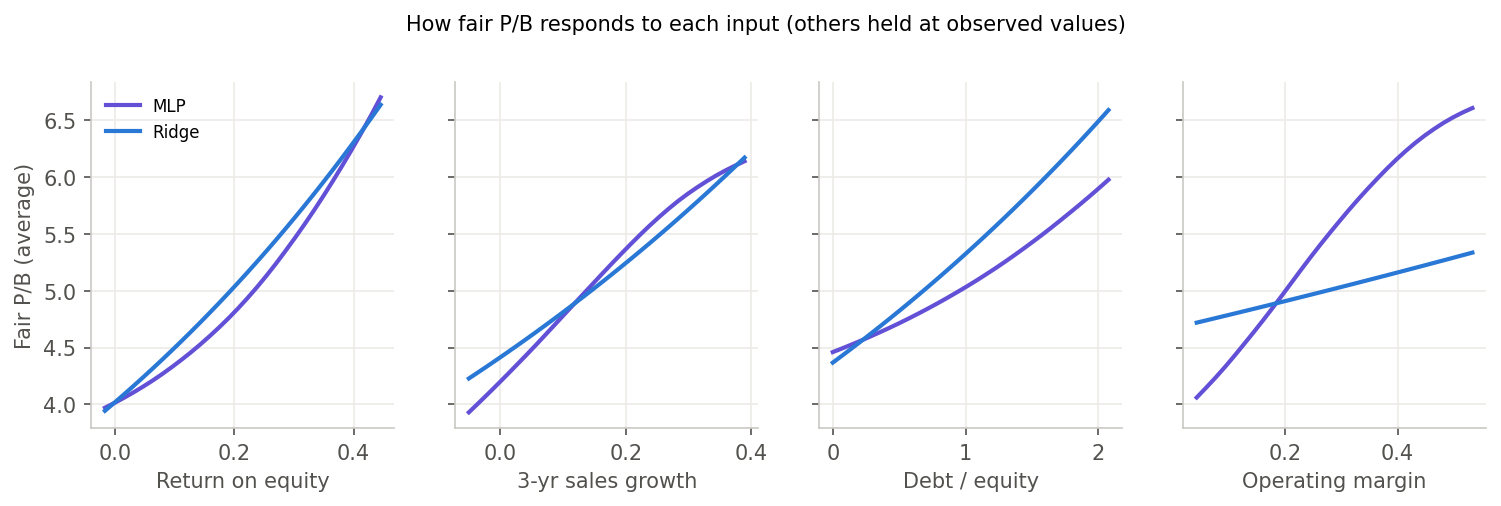
\includegraphics[width=0.9\textwidth]{fig7_partial_dependence.png}
\caption{Partial dependence of fair P/B on four inputs, other inputs held at their observed values.}
\label{fig:pdp}
\end{figure*}

\subsection{Valuing Companies the Model Has Not Seen}
The walk-forward test predicts next year's P/B for companies that already appear in earlier training years. Table~\ref{tab:robust}(c) reports the harder test relevant to valuing an unlisted business, in which each company is predicted by a model trained only on other companies. All models lose accuracy, but the ordering changes: XGBoost reaches 0.610, the MLP 0.577 and Ridge 0.560. So the MLP's walk-forward advantage comes partly from having seen a company before, whereas the tree ensemble's rules transfer better to new firms.

\subsection{Does Mispricing Predict Returns?}
It does not in this sample (Table~\ref{tab:bt}, Fig.~\ref{fig:bt}). Using the MLP, the IC between cheapness and the next 12-month return was positive in only two of seven years, with a mean of $-0.06$ ($t=-0.86$). The cheapest quintile returned 35.1\% a year on average and the most expensive 34.7\%, against 32.8\% for all stocks equally weighted. Ridge-based mispricing performed slightly better (mean IC $+0.03$, $t=0.43$, positive in four years, with a quintile spread of 9.1 percentage points), but not significantly.

\begin{table}[t]
\caption{Investment test: next 12-month price return by MLP mispricing}
\label{tab:bt}
\centering
\footnotesize
\begin{tabular}{@{}lccccc@{}}
\toprule
Formation & IC & Cheapest & Dearest & All & NIFTY \\
 & & 20\% & 20\% & stocks & 50 \\
\midrule
Jun 2019 & $-$0.326 & $-$17.3\% & 4.9\% & $-$1.0\% & $-$12.6\% \\
Jun 2020 & $-$0.027 & 98.7\% & 101.8\% & 95.9\% & 52.6\% \\
Jun 2021 & $-$0.140 & 6.0\% & 17.4\% & 6.4\% & 0.4\% \\
Jun 2022 & 0.195 & 49.4\% & 18.2\% & 33.8\% & 21.6\% \\
Jun 2023 & 0.146 & 113.1\% & 78.3\% & 84.9\% & 25.1\% \\
Jun 2024 & $-$0.070 & 2.5\% & 6.0\% & 4.8\% & 6.3\% \\
Jun 2025 & $-$0.199 & $-$6.9\% & 16.5\% & 4.4\% & $-$6.5\% \\
\midrule
Mean & $-$0.060 & 35.1\% & 34.7\% & 32.8\% & 12.4\% \\
\bottomrule
\end{tabular}
\end{table}

\begin{figure}[t]
\centering
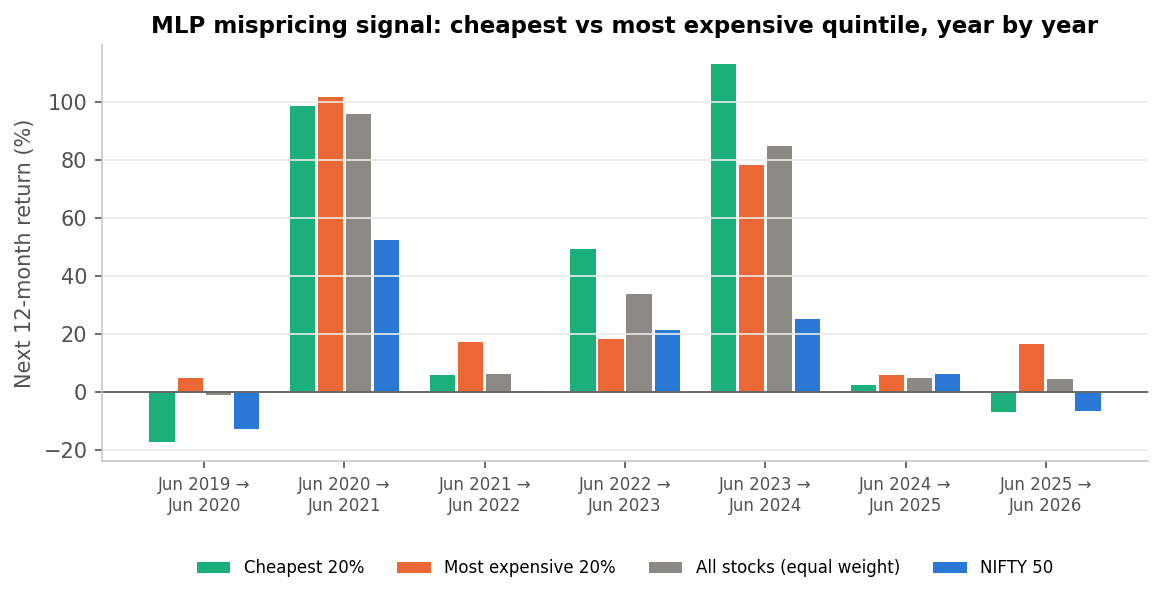
\includegraphics[width=\columnwidth]{fig8_backtest.png}
\caption{Next 12-month return of the cheapest and most expensive quintiles by MLP mispricing, against all stocks and the NIFTY~50.}
\label{fig:bt}
\end{figure}

The residual is also persistent: a company's Ridge mispricing has a correlation of 0.81 with its value a year earlier, and 0.57 for the MLP. Stocks that look expensive relative to their accounts tend to remain expensive, which suggests that the residual reflects lasting company characteristics rather than errors that correct within a year.

\section{Discussion}
Accounting fundamentals and sector explain roughly two-thirds of the cross-sectional variation in P/B among Indian large caps, and a tuned neural network improves on a linear model by about 14 percentage points. Its lead over XGBoost is small for a single training run and becomes visible only when ten seeds are averaged. Tree ensembles usually dominate on tabular data~\cite{grinsztajn2022}, so this result was not expected. A likely reason is that valuation responds smoothly to profitability and growth, a shape that a moderately regularised two-layer network fits well.

Performance also depends heavily on tuning and, to a lesser degree, on the seed. The L2 penalty and width mattered most, the optimiser hardly at all, and a single seed overstated the network's accuracy by about 1.4 points of R\textsuperscript{2}. Averaging several seeds~\cite{lakshminarayanan2017} costs little and should be standard practice when results are reported.

Which model is best depends on the task. For valuing companies already in the data, the MLP leads; for valuing a company the model has never seen, which is the case for an unlisted business, XGBoost generalises better. For private-company valuation, a practitioner should rely on the tree ensemble, or on both models together. For investing, ``cheap'' in this framework does not mean ``undervalued''. Geertsema and Lu~\cite{geertsema2023} found that machine-learned mispricing predicted the next month's return for US stocks; over 12-month horizons for Indian large caps we find no reliable effect. The persistence of the residual suggests that it captures factors that annual accounts miss, such as brand strength, governance, expected growth and perceived quality~\cite{asness2019}. The fair-value model is more useful as a screen that asks what would have to be true to justify a given price than as a trading signal.

These conclusions agree with a preliminary pilot study we conducted on 20 NIFTY~50 companies using Screener.in data, in which the MLP also outperformed Ridge, last year's P/B was the strongest benchmark and mispricing did not predict returns. The larger Prowess sample makes the comparisons considerably more reliable.

\textbf{Limitations.} The universe is the current NIFTY~200, so survivorship bias remains despite the size rule; the equal-weighted average return of 32.8\% a year, far above the NIFTY~50's 12.4\%, reflects this. Returns are price returns and exclude dividends. Market capitalisation is June's monthly average rather than the 30~June value. The sample begins in 2017 because earlier abridged statements are sparse, and the investment test has only seven yearly observations. Finally, asset turnover and P/B share a balance-sheet denominator, so part of its importance may be mechanical.

\section{Reproducibility}
The notebook, outputs and paper are available at \url{https://github.com/SanketGore/AMLBT_Project}. The Prowess extracts are licensed to GIM by CMIE and are not redistributed; the repository documents every field, filter and file layout, with SHA-256 checksums, so that licensed users can verify their copy and others can rebuild comparable inputs from public filings and exchange prices. Every number in this paper comes from one run of \texttt{Fair\_Value\_NN\_Prowess.ipynb}, which writes all tables and figures to the \texttt{outputs/} folder. To reproduce them, place the data files in \texttt{data/prowess\_raw/}, open the notebook in Google Colab or Jupyter and choose \emph{Run all}. The notebook first checks the nine Prowess files against their SHA-256 checksums and needs no further internet access. Seeds are fixed (42 for the main run and 0--9 for the seed study), and all models run on a single thread. At the end, the notebook hashes the key result tables into a fingerprint and reports whether it matches the previous run. The run reported here used Python 3.13.18, NumPy 2.4.6, pandas 2.2.3, scikit-learn 1.6.1 and XGBoost 3.4.1 on Google Colab, and produced the fingerprint \texttt{cc76887f\ldots}. Different library versions can change the last decimal places but not the findings.

\subsection{AI Use Declaration}
Claude (Anthropic) was used to propose the project design, assist with data extraction from CMIE Prowess and Screener.in, write the notebook code, help interpret the results and draft the text of this paper from the outputs. The authors chose the problem and its scope, ran the pipeline, reviewed the outputs and checked every figure and table against the notebook.

\section{Conclusion}
This study examined what the Indian market pays for in its largest non-financial companies. Using 1,102 company-years from CMIE Prowess, we find that accounts and sector explain about 70\% of the out-of-sample variation in P/B with a tuned neural network, compared with 68\% for XGBoost and 56\% for a linear model. The network's advantage depends on regularisation and width and holds reliably only when several seeds are averaged. For companies outside the training data, XGBoost generalises best. The part of valuation that fundamentals cannot explain is persistent and did not predict returns over 2019--2025: stocks that appeared expensive relative to their accounts generally performed as well as those that appeared cheap.

The practical result is a reproducible fair-value model that is accurate enough to compare listed companies and to provide a starting multiple for an unlisted business, and the comparisons show which algorithm suits each use. Further work could use historical index constituents to remove survivorship bias, include dividends in returns, and test EV/EBITDA as an alternative target that does not share a denominator with the inputs.

\begin{thebibliography}{00}
\bibitem{ohlson1995} J.~A. Ohlson, ``Earnings, book values, and dividends in equity valuation,'' \textit{Contemp. Account. Res.}, vol.~11, no.~2, pp.~661--687, 1995.
\bibitem{penman1996} S.~H. Penman, ``The articulation of price-earnings ratios and market-to-book ratios and the evaluation of growth,'' \textit{J. Account. Res.}, vol.~34, no.~2, pp.~235--259, 1996.
\bibitem{bhojraj2002} S.~Bhojraj and C.~M.~C. Lee, ``Who is my peer? A valuation-based approach to the selection of comparable firms,'' \textit{J. Account. Res.}, vol.~40, no.~2, pp.~407--439, 2002.
\bibitem{damodaran2012} A.~Damodaran, \textit{Investment Valuation}, 3rd~ed. Hoboken, NJ, USA: Wiley, 2012.
\bibitem{rhodes2005} M.~Rhodes-Kropf, D.~T. Robinson, and S.~Viswanathan, ``Valuation waves and merger activity: The empirical evidence,'' \textit{J. Financ. Econ.}, vol.~77, no.~3, pp.~561--603, 2005.
\bibitem{gu2020} S.~Gu, B.~Kelly, and D.~Xiu, ``Empirical asset pricing via machine learning,'' \textit{Rev. Financ. Stud.}, vol.~33, no.~5, pp.~2223--2273, 2020.
\bibitem{geertsema2023} P.~Geertsema and H.~Lu, ``Relative valuation with machine learning,'' \textit{J. Account. Res.}, vol.~61, no.~1, pp.~329--376, 2023.
\bibitem{grinsztajn2022} L.~Grinsztajn, E.~Oyallon, and G.~Varoquaux, ``Why do tree-based models still outperform deep learning on typical tabular data?'' in \textit{Proc. NeurIPS Datasets and Benchmarks Track}, 2022.
\bibitem{chen2016} T.~Chen and C.~Guestrin, ``XGBoost: A scalable tree boosting system,'' in \textit{Proc. 22nd ACM SIGKDD}, 2016, pp.~785--794.
\bibitem{breiman2001} L.~Breiman, ``Random forests,'' \textit{Mach. Learn.}, vol.~45, no.~1, pp.~5--32, 2001.
\bibitem{bergstra2012} J.~Bergstra and Y.~Bengio, ``Random search for hyper-parameter optimization,'' \textit{J. Mach. Learn. Res.}, vol.~13, pp.~281--305, 2012.
\bibitem{bouthillier2021} X.~Bouthillier et al., ``Accounting for variance in machine learning benchmarks,'' in \textit{Proc. MLSys}, 2021.
\bibitem{lakshminarayanan2017} B.~Lakshminarayanan, A.~Pritzel, and C.~Blundell, ``Simple and scalable predictive uncertainty estimation using deep ensembles,'' in \textit{Proc. NeurIPS}, 2017.
\bibitem{hoerl1970} A.~E. Hoerl and R.~W. Kennard, ``Ridge regression: Biased estimation for nonorthogonal problems,'' \textit{Technometrics}, vol.~12, no.~1, pp.~55--67, 1970.
\bibitem{pedregosa2011} F.~Pedregosa et al., ``Scikit-learn: Machine learning in Python,'' \textit{J. Mach. Learn. Res.}, vol.~12, pp.~2825--2830, 2011.
\bibitem{fisher2019} A.~Fisher, C.~Rudin, and F.~Dominici, ``All models are wrong, but many are useful: Learning a variable's importance by studying an entire class of prediction models simultaneously,'' \textit{J. Mach. Learn. Res.}, vol.~20, no.~177, pp.~1--81, 2019.
\bibitem{friedman2001} J.~H. Friedman, ``Greedy function approximation: A gradient boosting machine,'' \textit{Ann. Statist.}, vol.~29, no.~5, pp.~1189--1232, 2001.
\bibitem{asness2019} C.~S. Asness, A.~Frazzini, and L.~H. Pedersen, ``Quality minus junk,'' \textit{Rev. Account. Stud.}, vol.~24, no.~1, pp.~34--112, 2019.
\end{thebibliography}

\end{document}
